
%%%%%%%%%%%%%%%%%%%%%%%%%%%%%%%%%%%%%%%%%%%%%%%%%%%%%%%%%%%%%%%%%%%%%%%%
%Para las ecuaciones siempre es Ec.(n).
%Para las figuras siempre es Fig.n, incluso en el caption de la figura. Tambien las Tablas
%Para las referencias es [n]
%%%%%%%%%%%%%%%%%%%%%%%%%%%%%%%%%%%%%%%%%%%%%%%%%%%%%%%%%%%%%%%%%%%%%%%%

\documentclass[
reprint,
%notitlepage,
%superscriptaddress,
%groupedaddress,
%unsortedaddress,
%runinaddress,
%frontmatterverbose, 
%preprint,
%showpacs,preprintnumbers,
%nofootinbib,
%nobibnotes,
%bibnotes,
%11 pt,
amsmath,
amssymb,
aps,
pra,
%prb,
%rmp,
%tightenlines %esto hizo el milagro de sacar los espacios en blancos estocásticos (?)
 %prstab,
%prstper,
%floatfix,\textbf{}
]{revtex4-1} %Instalar primero para usarlo. Paquete malo.

%\documentclass[onecolumn, aps, amsmath,amssymb ]{article}
\usepackage{lipsum}  
\usepackage{graphicx}% Include figure files
\usepackage{subfig}
\usepackage{braket}
\usepackage{comment} %comment large chunks of text
\usepackage{dcolumn}% Align table columns on decimal point
\usepackage{bm}% bold math
%\usepackage{hyperref}% add hypertext capabilities
\usepackage[mathlines]{lineno}% Enable numbering of text and display math
%\linenumbers\relax % Commence numbering lines
\usepackage{mathtools} %% Para el supraíndice

\usepackage[nice]{nicefrac}

%%%%%%%El Señor Español%%%%%%%%%%%%%%%%%%%%%%%%%%%
\usepackage[utf8]{inputenc} %acento
\usepackage[
spanish, %El lenguaje.
es-tabla, %La tabla y no cuadro.
activeacute, %El acento.
es-nodecimaldot %Punto y no coma con separador de números
]{babel}
\usepackage{microtype} %para hacerlo más bonito :33 como vos (?) 
%%%%%%%%%%%%%%%%%%%%%%%%%%%%%%%%%%%%%%%%%%%%%%%%%%%
%%%%%%%%% Para que las imágenes se queden dónde las quiero (?
\usepackage{float}
%%%%%%%%%%

%%%%%%%%Cambia a Fig de Figure%%%%%%%%%%
\makeatletter
\renewcommand{\fnum@figure}{Fig. \thefigure} 
\makeatother
%%%%%%%%%%%%%%%%%%%%%%%%%%%%%%%%%%%%%%%%
\raggedbottom


\begin{document}
%%%%%%%%%%%%%%%%%%%%%%%%%%%%%%%%%%Título%%%%%%%%%%%%%%%%%%%%%%%%%%%%%%%%%%%%%%
%%%%%%%%%%%%%%%%%%%%%%%%%%%%%%%%%%%%%%%%%%%%%%%%%%%%%%%%%%%%%%%%%%%%%%%%%%%%%%

\title{Práctica 6: Memorias Asociativas}
\author{Evelyn~G.~Coronel}

\affiliation{
Redes Neuronales - Instituto Balseiro\\}

\date[]{\lowercase{\today}} %%lw para lw, [] sin date


\maketitle
%%%%%%%%%%%%%%%%%%%%%%%%%%%%%%%%%%%%%%%%%%%%%%%%%%%%%%%%%%%%%%%%%%%%%%%%%%%%%%%%%%%
% Podemos usar cualquiera de los dos comandos: \input o \include para incluir el texto
%\input{./Capitulo1/cap1.tex}

\subsection*{Cuestiones generales del modelo  de Hopfield}

El modelo de Hopfield contempla la idea de solucionar de la manera más simple el problema de memorizar patrones. Este problema consiste en memorizar un conjunto de patrones $\xi^\mu _i$, de tal manera que si se presenta un patrón $\zeta^\mu_i$, la red responde con el patrón almacenado que más se parece a la entrada dada \cite{hertz}.

La red almacena $p$ patrones, que se indexan con $\mu=1, \dots, p$, mientras que las unidades dentro de la red se indexan mediante $i=1, \dots, N$. La convención que se toma en este trabajo es que cada patrón $\xi^\mu _i$ puede valer $+1$ o $-1$.
\subsubsection*{Sobre la actualización}

Se toma una regla de actualización asincrónica, esta implica que:

\begin{itemize}
	\item En cada época, se selecciona una unidad i a ser actualizada aplicando la regla de la Ec.\,(\ref{hop_noiseless})
	\item Cada unidad elige independientemente actualizarse o no, con una probabilidad en cada época. 
\end{itemize}

Para el modelo de Hopfield sin ruido, la probabilidad es constante en cada actualización es igual a $0.5$, es decir, se actualiza a cada paso con $+1$ o con $-1$. En cambio, para el modelo de Hopfield con ruido, la probabilidad de cambio está dada por una función que depende de la salida $h_i$ y de otro parámetro que simula un ruido térmico $T$.

\subsubsection*{Salida de la red  para varios patrones}

Se define la matriz de conexiones $w_{ij}$, análoga a una una matriz de pesos, según la Ec. \ref{pesos}.
\begin{equation}
	w_{ij} = \frac{1}{N} \sum _{\mu=1} ^{p}\xi_i^\mu \xi_j^\mu 
	\label{pesos}
\end{equation}
donde el índice $i, j= 1, \dots , N$ recorre las unidades de la red y el índice $\mu= 1, \dots, p$ recorre el conjunto de patrones.

Dada una entrada $\zeta ^\mu_i$, definamos el parámetro $h^\nu_i $ como $h^\nu_i = \sum_j w_{ij} \zeta_j ^\nu$. Para la validación de las redes de esta práctica, se utilizaron los mismos patrones almacenados en la matriz de conexiones como entradas a la red. 

\section*{Ejercicio I: El modelo de Hopfield sin ruido}

Definamos el parámetro de carga $\alpha  = \nicefrac{p}{N}$, que es el número de patrones a almacenar como fracción de la cantidad de unidades por patrón.  Para el caso del modelo de Hopfield sin ruido, se espera que exista un valor de $\alpha$ crítico, con un valor de  $\alpha_c \approx 0.138$, donde la red pierde su capacidad de memorizar patrones.

Para el modelo de Hopfield sin ruido, alimentando la entrada con un patrón $\xi_i^\nu$, la primera iteración se realiza la siguiente operación:
\begin{equation}
	S_i := sgn(h^\nu _i- \theta_i)
\end{equation}
donde $sgn(x)$ es la función signo y para este trabajo $\theta_i = 0$. Para el siguiente paso, se toma como entrada los valores de $S_i$ de la iteración anterior y se actualizan según la regla de la Ec.\ref{hop_noiseless} hasta que el sistema alcanza la condición de la Ec.\ref{converg}, conocida como condición de estabilidad.
\begin{align}
	\text{Cada iteraci\'on }S_i &:= sgn(h^\nu _i), \label{hop_noiseless}\\	
	\text{Converge cuando }S_i &:= sgn(h^\nu _i) \quad \forall \,i \label{converg}
\end{align}

Posteriormente, después que el sistema converge, se calcula el overlap $m^\mu$ como
\begin{equation}
	m^\mu = \frac{1}{N} \sum^N_i S_i \xi^\mu_i
\end{equation}
donde $\xi^\mu_i$ es el patrón que se usó como condición inicial y $S_i$ es el valor al que convergió el sistema.

\subsection{Resultados}

Se utilizaron valores de $N=500, 1000, 2000, 4000$ con valores  de $\alpha=0.12, 0.14, 0.16, 0.18$, tomando un patrón como condición inicial e iterando el sistema hasta alcanzar la condición de estabilidad de la Ec.\,\ref{converg}. Para posteriormente calcular $m^\mu$ y obtener su distribución para una cantidad de patrones $N_{patrones}$, con $N$ y $\alpha$ fijos. Estos histogramas se muestran en las Figs.\,\ref{fig:500}, \ref{fig:1000}, \ref{fig:2000} y \ref{fig:4000} para un ancho de bin de $0.05$.


Haciendo una analogía con un sistema de espines, consideremos que $N$ se corresponde con el tamaño, donde $N\times N$ es el tamaño de la red. Para distintos tamaños y para $\alpha=0.12$, se observa que la mayor parte de los overlaps es cercano a $1$. Esto indica que el sistema puede reconocer los patrones que se almacenaron en la matriz de conexiones. En cambio, a partir de $\alpha=0.14$, para los tamaños estudiados, el histograma tiene una componente alrededor de $0.4$. Por que el valor de $\alpha_c \approx 0.138$ es consistente con simulación.

\begin{figure}[H]
	\centering
	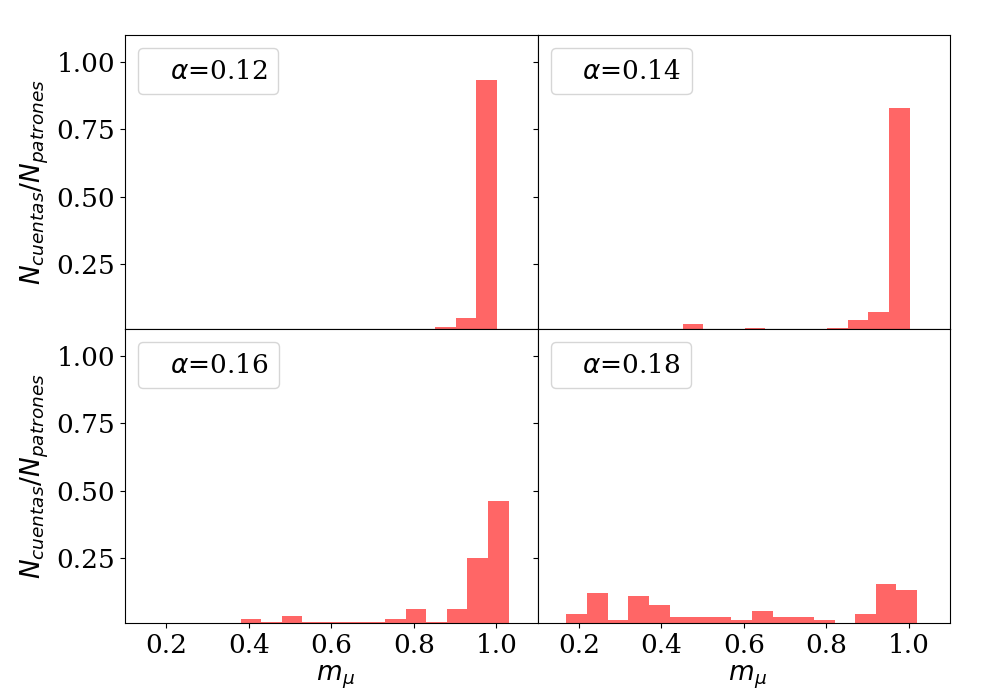
\includegraphics[width=0.5\textwidth]{../Graficos/500.png}
	\caption{Para $N=500$}
	\label{fig:500}
\end{figure}
\begin{figure}[H]
	\centering
	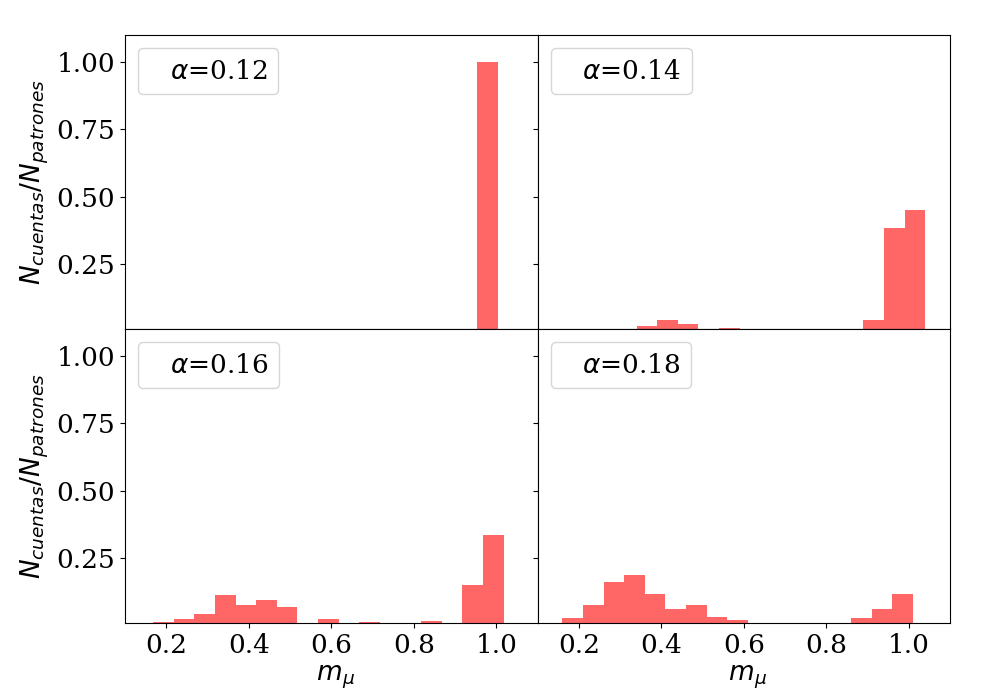
\includegraphics[width=0.5\textwidth]{../Graficos/1000.png}
	\caption{Para $N=1000$}
	\label{fig:1000}
\end{figure}
A medida que aumenta el valor de $\alpha$, la componente del histograma en la región de $m^\mu \approx 0.3$ también aumenta. Esto es consecuencia de que pasamos el valor de $\alpha_c$, donde la red ya  no puede reconocer los patrones con los que estamos alimentando la entrada, es decir que el sistema ya no puede almacenar patrones para está cantidad de patrones.


Para el valor más alto de $\alpha$ estudiado, se observan distintos comportamientos del histograma para distintos tamaños de red. Comparando las Figs.\,\ref{fig:500} y \ref{fig:4000}, donde para $N=500$ se observa que el sistema reconoce aproximadamente un $20\,\%$ de los patrones presentados, en cambio para $N=4000$ el sistema no es capaz de almacenar ninguno de  patrones utilizados para la verificación del sistema.
\begin{figure}[H]
	\centering
	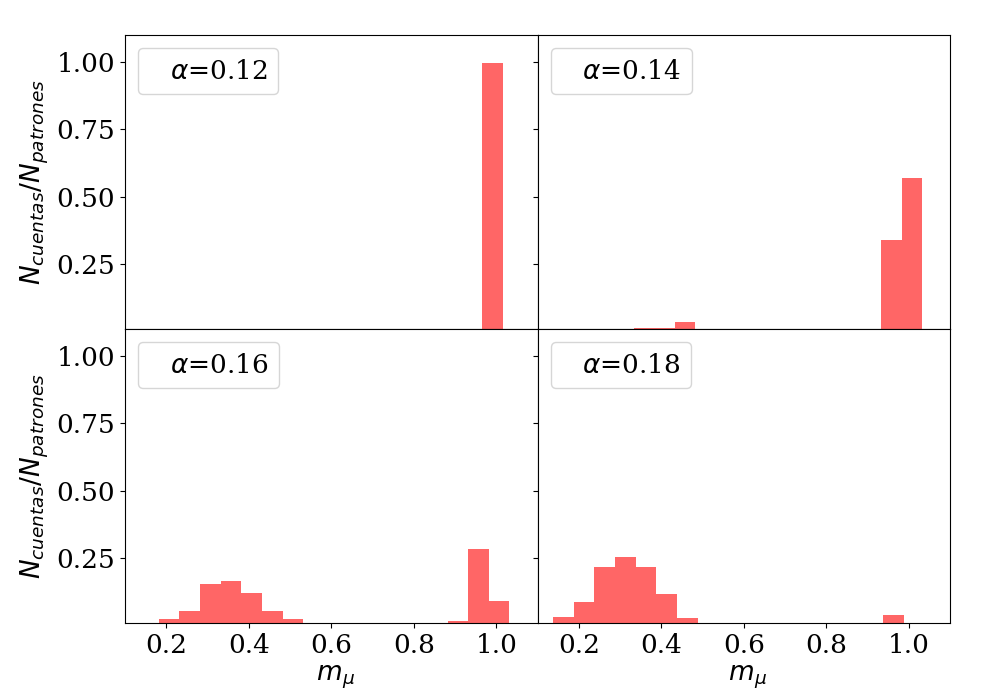
\includegraphics[width=0.5\textwidth]{../Graficos/2000.png}
	\caption{Para $N=2000$}
	\label{fig:2000}
\end{figure}
\begin{figure}[H]
	\centering
	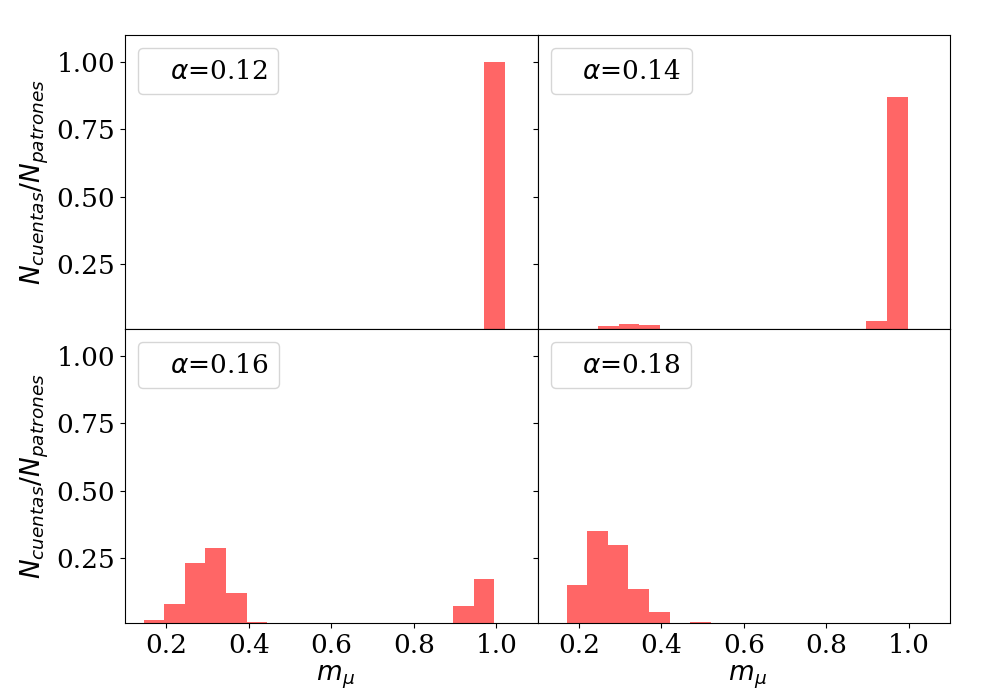
\includegraphics[width=0.5\textwidth]{../Graficos/4000.png}
	\caption{Para $N=4000$}
	\label{fig:4000}
\end{figure}

Otro aspecto en particular de los histogramas por encima de $\alpha_c$, es que se espera que el overlap sea nulo, en cambio se observa que sistema converge a un valor de aproximadamente $0.3$. 

\subsection{Modificaciones a los pesos}
En este caso, las conexiones entre unidades son $\pm 1$, manteniendo el signo del valor de la definición \ref{pesos}.  Para $N=1000$ y para $\alpha= 0.05, 0.09, 0.1, 0.12$, como se muestra en la Fig.\ref{fig:1000_alpha}. Se observa que al cambiar los pesos a variables enteras $\pm 1$, el $\alpha_c$ está entre $0.1$ y $0.12$, por lo que disminuyó ligeramente con respecto al caso anterior.

La ventaja de este algoritmo sobre el caso anterior es que se necesita menos memoria para almacenar la matriz de conexiones, ya que solo son dos valores enteros. Entonces la memoria de la máquina que realiza la simulación puede asociarse a un solo bit a cada entrada del matriz $w_{ij}$\cite{hertz}.


\begin{figure}[H]
	\centering
	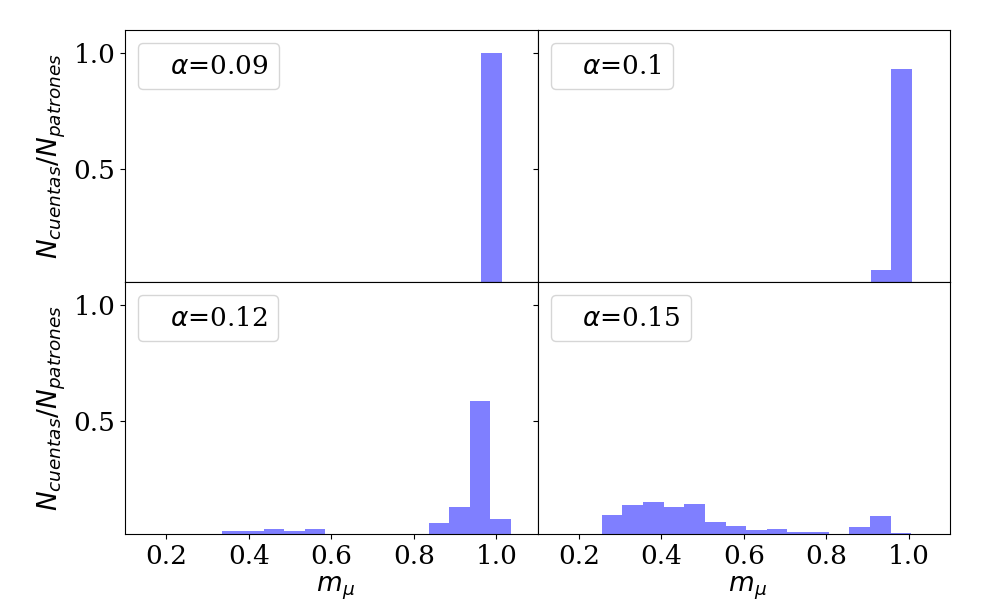
\includegraphics[width=0.485\textwidth]{../Graficos/1000_alpha.png}
	\caption{Para $N=1000$ y los pesos modificados}
	\label{fig:1000_alpha}
\end{figure}
\section*{Ejercicio II: El modelo de Hopfield con ruido}

Para el análisis de esta sección, utilizamos la analogía a un sistema de espines. En el modelo de Hopfield con ruido tiene una diferencia a la hora de la actualización de los $S_i$. En este caso, tenemos la regla de actualización dada por la Ec.\,\ref{ruido}.
\begin{align}
	S(t+1)_i=  \begin{cases} 
   +1 & \text{Probabilidad }P(h_i, t, +1) \\
   -1 & \text{Probabilidad }P(h_i, t, -1) 
\end{cases},
\label{ruido}
\end{align}
\begin{equation}
	P(h_i, t, \pm 1) = \frac{\exp{(\pm \beta h_i(t))}}{\exp{(- \beta h_i(t))} +\exp{(\beta h_i(t))}}
	\label{prob}
\end{equation}
donde  la ecuación de $P(h_i, t, \pm1)$ viene dada por la Ec.\,\ref{prob}. Nótese que $P(h_i, t, +1) + P(h_i, t, -1) =1$. El parámetro $\beta$ es inversamente proporcional al nivel de ruido del sistema. Para la implementación del algoritmo, se toma un número $P_{ref}$ con distribución uniforme entre 0 y 1, y se compara con $P(h_i, t, +1)$, si  $P(h_i, t, +1) \ge P_{ref}$ se hace el cambio a $+1$, caso contrario a $-1$.


\subsubsection{Resultados}

Tomando los parámetros iguales a $N=4000$, $p=40$ y $N=1000$ con $p=100$,  para temperaturas $T$ en el rango $[0.1, 2.0]$, tomando como $k_B=1$ por lo que $\beta=\nicefrac{1}{T}$. El resultado de las simulaciones en función de la temperatura se muestran en la Fig.\,\ref{fig:T}.
\begin{figure}[H]
	\centering
	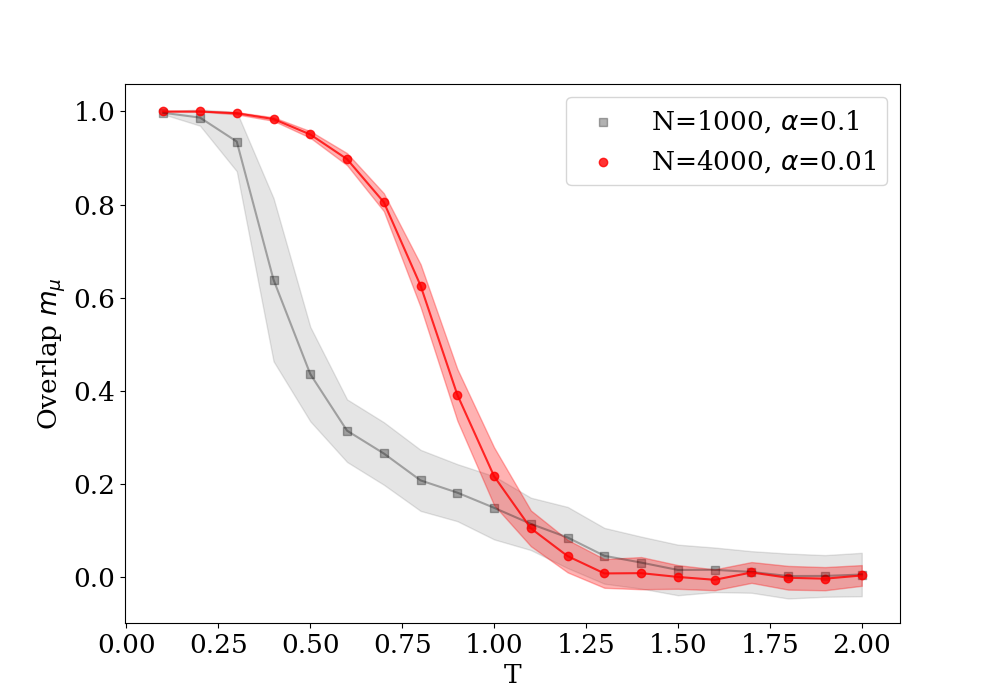
\includegraphics[width=0.5\textwidth]{../Graficos/beta2.png}
	\caption{El overlap en función de $T$}
	\label{fig:T}
\end{figure}
En la Fig. \ref{fig:T} se ve que para temperaturas bajas, el overlap de la red es cercana a 1, pero a medida que aumenta el ruido térmico la red empieza a perder la capacidad de almacenar  patrones.  Dependiendo del valor de $\alpha$ del sistema, la temperatura a la que pierde esta capacidad es distinta. Mediante estas dos simulaciones se ve que a menor $\alpha$, mayor es la temperatura donde ocurre el quiebre en $m_\mu$ en función de $T$. 

\bibliography{hertz} 



\end{document}